\section{Optimization theory}
\label{Optimization_theory}
The following section describes the basic theory of software optimization. First, I will summarize guidelines that should always be followed when one has to optimize a piece of software. Naturally, these will only be a selection of the advice provided by relevant manuals. Then, I will go into detail when explaining concepts of using the SSE instruction set. The section is completed by a small remark on compiler optimization. While the advice given in this section is focussed on C/C++ code, most of them should be valid for other programming languages as well.

\subsection{Basic principles}
The first lesson a programmer learns when looking into software optimization is to \emph{avoid premature optimization}. This advice is based on a statement given by Donald E. Knuth in~\cite{knuth1974}, ``We \emph{should} forget about small efficiencies, say about 97 \% of the time: premature optimization is the root of all evil''. Knuth continues to say that in the remaining (critical) 3 \% of the code the programmer should look carefully for optimization opportunities, ``but only \emph{after} that code has been identified''. The common notion of Knuth's words is that, while writing a piece of software, the programmer should not care about performance until he can guarantee the code's correctness. Afterwards, he should find the most critical parts in the code and concentrate optimization efforts on those particular parts. This opinion implies two valid points: First, optimized code will always reduce readability and increase complexity. This may lead to errors and code that is hard to maintain. Second, most of the time optimization is only worth its costs in the most time-critical parts of a software. However, Knuth supposedly did not mean that the programmer should not think about performance at all. In fact, some basic rules can be kept in mind along the way. 

In general, the performance of an application is either limited by processor speed or by memory bandwidth. Knowing which one will be the limiting factor in a particular piece of code can be helpful to avoid certain bottlenecks from the beginning. In order to design the code in a resource saving manner, it is critical for the programmer to understand the internals of these core system components. In the following I will present some information on modern (x86) microprocessor features and on how to write code that makes efficient use of both the processor and the memory. However, since this is not the main topic of my thesis and there is plenty of information on the net, I will single out only a few major items.

\subsubsection{CPU performance}
On modern processor architectures, the execution of an instruction is divided into several stages which are executed sequentially. To reiterate the textbook example (for example, see~\cite[p. 411]{murdocca1999computer}, consider the following model consisting of 4 stages: First, the instruction needs to be fetched (IF) from memory or from a code cache. Second, the instruction needs to be decoded (ID) and, third, executed (EX). At stage 4 the results of the instruction need to be written back to memory or registers (WB). When the instruction fetch unit finishes its work, it immediately starts fetching the next instruction from the code, the decoder starts decoding it and so on. Therefore, the instructions are literally processed in parallel. This staging of instructions and their parallel execution is called \emph{pipelining}. While in theory this model can complete the execution of one instruction every cycle, in practise it if often limited by data dependencies between the instructions. If an instruction depends on the results of a preceding instruction, it needs to wait for the results to be written back to registers, effectively stalling the processor. See Figure~\ref{fig:pipeline} for an example: Here, the second instruction depends on the result of the first and thus its execution has to be delayed. Note that in this example the EX stage requires only one clock cycle, which is only true for simple instructions such as addition or subtraction of integers.

\begin{figure}[h]
\begin{center}
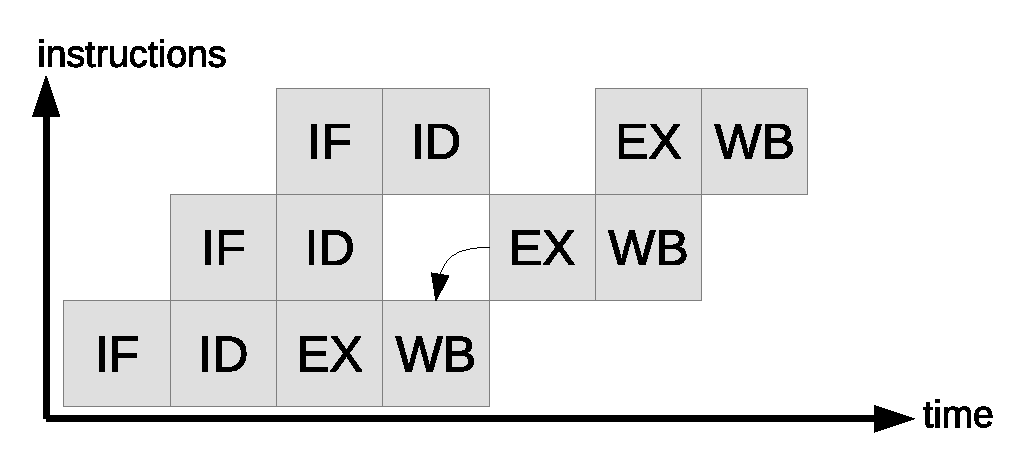
\includegraphics[width=0.5\textwidth]{img/pipeline}
\end{center}
\caption{Model of a filled processor pipeline with a data dependency}
\label{fig:pipeline}
\end{figure}

As most modern microprocessors have multiple execution units for various types of operations (e.g. the x87 floating point unit that's solely purpose is to process floating point calculations), or even have multiple units of the same type, instructions that are executed on different execution unit can be processed in parallel. This is known as \emph{out of order execution}, as the instructions do not necessarily need the same amount of clock cycles and a particular instruction may be outpaced by a succeeding faster instruction, i.e. the instructions are executed ``out of order''. Some modern processors may even reorder instructions on the same execution unit. Out of order execution, just like pipelining, suffers from data dependencies.

In general, data dependencies only measurably diminish performance when appearing in longer sequences (called \emph{dependency chains}), for example in loops. To minimize pipeline stalling, the programmer needs to reduce the number of data dependencies in such loops. Listing~\ref{unrolled} displays an example taken from Agner Fog's optimization manual~\cite[p. 103]{fog2011optimizing}. The increment operation on the loop variable \texttt{i} and the floating point operations are executed on different execution units and thus are likely to be executed out of order. Therefore, the bottleneck is the more expensive floating point addition. In version 1, every floating point addition depends on the result (\texttt{sum}) of the preceding addition, which stalls the pipeline. In constrast, in version 2, two succeeding additions do not depend on each other and thus do not cause a pipeline stall. The technique demonstrated here is known as \emph{loop unrolling}. It usually comes at the expense of additional instructions at the end of the loop (here: \texttt{sum1 += sum2;}), which can almost always be neglected.
\begin{code}[caption={Loop unrolling example}, label=unrolled]
const int size = 100;
float list[size]; int i;

// Version 1:
float sum = 0;
for (i = 0; i < size; i++) 
  sum += list[i];

// Version 2:
float sum1 = 0, sum2 = 0;
for (i = 0; i < size; i += 2) {
  sum1 += list[i];
  sum2 += list[i+1];
}
sum1 += sum2;
\end{code}

%Duffs device?

Another positive effect of loop unrolling is that the loop control branch is evaluated less often. This often leads to better branch prediction results resulting in fewer mispredicted conditional jumps (see Section~\ref{conditional_branches} for further explanation of conditional branches). Apart from loop unrolling, another simple technique to avoid data dependencies and make full use of out of order execution is known as \emph{instruction reordering} or \emph{instruction pairing}. Simply put, instructions that do not depend on each other should be grouped whereas instructions having dependencies between them should be interleaved with other unrelated instructions. For out of order execution it is also desirable to mix instructions which are using different execution units, for example integer and floating point operations. It may not always be easily visible if such measures truly affect the processing inside the CPU, since modern CPUs generally have sophisticated instruction scheduling features and thus ``outsmart'' the programmer. Additionally, performance impact may vary across different CPU generations, for example when newer CPUs contain further execution units. Hence, it is necessary to thoroughly benchmark any optimized code and decide whether these measures are worth the loss of readability, which can be especially bad in the case of instruction reordering.

\subsubsection{Memory performance}
\label{memory_performance}
\paragraph{Stack vs. heap storage of variables.} The memory of an application is divided into two major parts: The stack resides at the beginning of the memory block and is used in a last-in-first-out fashion. When an application allocates a variable on the stack (i.e., all local variables in C), it simply needs to move up the \emph{stack pointer}. The heap usually resides at the end of the memory, growing down. It is used for dynamic memory allocation. When the application wants to allocate memory on the heap, for example because it wants to allocate a dynamically sized array, it needs to ask a heap manager for it (\texttt{malloc} in C). This manager would then look for a storage position that provided sufficient free space for the variable. Managing the heap is much more expensive compared to the simple stack approach, yet it may sometimes be impossible to store all variables on the stack. For instance, in some older programming languages such as C89, it was not allowed to allocate memory on the stack when the size was not known at compile time. Apart from that, the stack is much smaller than the heap and some objects or large arrays may exceed its space limits. However, as the dynamic allocation overhead and additionally the potential memory fragmentation resulting from it reduce performance perceivably, frequently used variables should be stored on the stack whenever possible~\cite[p. 90]{fog2011optimizing}.

\paragraph{Cache misses.} Modern microprocessor architectures feature a multi-level hierarchy of caches which is used to speed up repeated accesses to data values. The Level 1 cache, being the (physically) closest cache available to the CPU, provides the fastest access time. With every successive cache (L2/L3), both access times and cache size increase. For simplicity, I will assume a model of only one cache in the following. Whenever an application uses or manipulates a variable, the CPU checks whether the memory segment where it resides is already loaded into the cache. It if is not, a \emph{cache miss} occurs, resulting in the segment being fetched from main memory. Since the RAM is extremely slow compared to the CPU, the latter is a very time-consuming operation\footnote{In fact, memory access times depend on the internal clockings of the memory modules integrated in the computer as well as the clock frequency of the \emph{Front Side Bus} (FSB), which connects it to the CPU. In ``Principles of Computer Architecture''~\cite[p. 256]{murdocca1999computer} the access time is specified as 60-80 nanoseconds, whereas a register access costs only 1 nanosecond. Although the book is from the late 1990s and the data is likely to be outdated, the proportion should be still valid today.}. The programmer's goal is to reduce the number of cache misses his code produces. The main motivation for today's cache architectures is the so-called \emph{locality of reference} or \emph{data locality}. Technically, data locality refers to probability observations about data access patterns, that are commonly divided into two types: First, temporal locality means that data that has been accessed recently is very likely to be accessed again soon. Second, spatial locality means that data that is spatially close to recently accessed data with regards to its position in the memory (i.e., the memory addresses are similar) is likely to be accessed soon, too. Therefore it makes sense to not only cache a single variable that was recently used, but the whole memory range where this variable resided. Now, to exploit the CPU's caching mechanism, the programmer should adapt his access patterns to these probability estimations. As Agner Fog puts it, ``Variables that are used together should be stored together''~\cite[p. 88]{fog2011optimizing}. This boils down to simple strategies such as always allocating variables when one needs them. As an often used example for cache-friendly variable access, consider the array manipulation in Listing~\ref{seq_array_access}.
\begin{code}[caption={Sequential vs. non-sequential array access}, label=seq_array_access]
int buf[1024 * 1024];

for (int i = 0; i < 1024; i++)
  for (int j = 0; j < 1024; j++)
    buf[i * 1024 + j]++;

for (int i = 0; i < 1024; i++)
  for (int j = 0; j < 1024; j++)
    buf[j * 1024 + i]++;
\end{code}

While both nested loops do the same thing, namely increment each element in the buffer, the crucial difference between them is the way the array index is calculated. While the first loop walks through the array sequentially with the index always growing by one, the second loop ``jumps'' through the array in steps of 1024. The second approach results in a lot more cache misses, as the cache lines get repeatedly displaced by others.

\subsection{Parallelization using Streaming SIMD Extensions}
Created to meet the growing demand for fast multimedia functions in 1996, Intel's MMX technology was the first widely used instruction set extension to deploy the SIMD architecture to modern desktop processors. It used the lower 64 bit of the 80 bit x87 floating point registers to allow for vectorized calculation of 8 bit to 64 bit integers using special SIMD instructions. Its successor, the Streaming SIMD Extensions (SSE), first added 8 separate 128 wide registers for vector calculations (\texttt{xmm0} to \texttt{xmm7}), later complemented by another 8 (\texttt{xmm8} to \texttt{xmm15}) by SSE4. Besides, SSE introduced the possibility to process 4 single or 2 double precision floating point values, on which I will concentrate in the following. Most recently, Intel and AMD have begun to produce new processor lines that include support for the so-called Advanced Vector Extensions (AVX), which can be considered the legal successor of SSE4. The main advantage of AVX over SSE4 is the introduction of 256 bit wide registers and corresponding instructions. Nevertheless, as AVX has only been available on the market for some months and has not changed much with regards to vectorized floating point C code, I will only focus on SSE. The reader may think ``AVX'' whenever I write ``SSE''.

SSE instructions on so-called \emph{packed values} are executed on multiple, physically existing execution units and hence need the same amount of clock cycles as their scalar counterparts. For example, on a 45nm Intel Core 2 processor, both the \texttt{ADDPS} SSE instruction and the \texttt{FADD} instruction have a throughput of 1 instruction per clock cycle~\cite[pp. 50, 57]{fog2011instructiontables}. Whereas \texttt{FADD} calculates the sum of 2 floating point values on the x87 floating point unit (FPU), \texttt{ADDPS} calculates the sums of 4 pairs of floating point values in two \texttt{xmm} registers. Listing~\ref{sse_assembler_intro} shows simplified assembler code that calculates the sum of an array of floats using SSE instructions. Note that this is AT\&T syntax, i.e. source operand before destination operand.
\begin{assembler}[caption={Array sum using simplified SSE assembly}, label=sse_assembler_intro]
  ; ecx contains the length of the array
  ; edx contains the address of the array

  movaps [edx], xmm0
LOOP1:
  add    0x10, edx
  movaps [edx], xmm1
  addps  xmm1, xmm0

  dec    ecx
  jnz    LOOP1

  haddps xmm0, xmm0
  haddps xmm0, xmm0
  movss  xmm0, ebx

  ; now ebx holds the sum of the floats
\end{assembler}

\texttt{movaps} (\texttt{mov}e \texttt{a}ligned \texttt{p}acked \texttt{s}ingle) moves 16 bytes (or 4 single precision floats) between memory and a \texttt{xmm} register. \texttt{addps} adds up 2 registers filled with packed single precision floats vertically. The most interesting part here is the SSE instruction found in lines 13 and 14: \texttt{haddps} horizontally adds adjacent elements in the two operand registers and stores the sums in the destination register, as can be seen in Figure~\ref{fig:haddps}. This illustrates that SSE code usually turns out to be considerably larger in size and number of instructions than scalar code, as the wrapping of data values into vectors (i.e., the ``packing'') and the un-wrapping again are distinct steps that only show up in vectorized code. In this case, the horizontal add would not be needed if the floats were added up one by one.

\begin{figure}[h]
\begin{center}
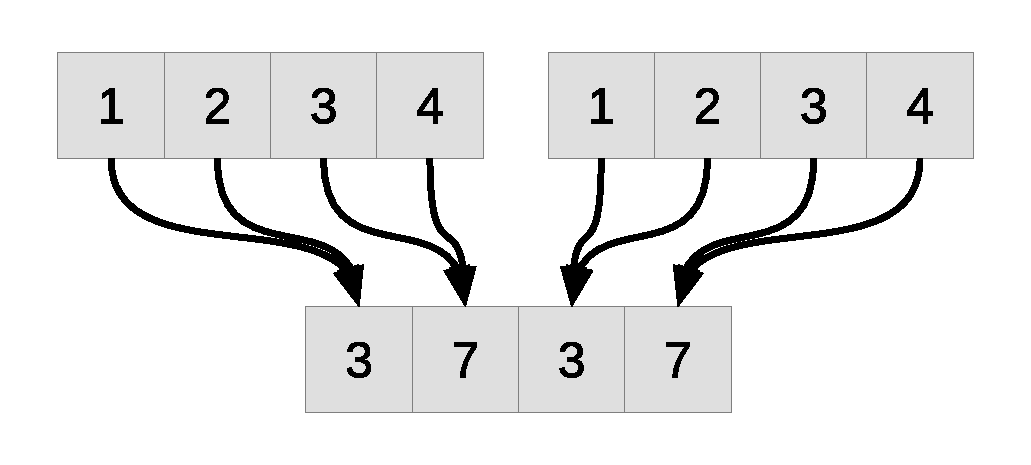
\includegraphics[width=0.5\textwidth]{img/haddps}
\end{center}
\caption{Horizontal Add Packed Single}
\label{fig:haddps}
\end{figure}

The theoretical speed-up factor when enriching scalar code with single precision floating point SSE instructions is limited by the maximum number of floats to be processed simultaneously, which is 4. The mentioned vectorization steps constitute a large enough overhead to easily reduce the speed-up to a factor of 3. However, this speed-up only applies to linear code without control flow statements depending on single data values. Since conditional branches (\texttt{if} statements and the like) inhibit data-parallel execution, they present a difficult to manage obstacle for SSE optimization that needs to be cleared by using special techniques such as blending (see section~\ref{conditional_branches}). These may sometimes impose a performance drawback that completely consumes the expected vectorization speed ups. In practise, my experiments with SSE and moderately complex code resulted in actual speed up factors between 1.5 and 2 (see Section~\ref{Evaluation}).

\subsection{Techniques for programming with SSE}
Fortunately, programming with SSE is well supported by modern compilers. Nowadays, there is no need to use inline assembler at all, as Intel, since the very beginning of MMX and SSE, provided specifications for \emph{compiler intrinsics} for C/C++ languages along the SSE specifications. These intrinsics can be used to instruct the compiler to emit a specific SSE instruction, although the compiler is not obliged to actually comply with the programmer's request. For a start, there were two data types defined that help mixing SSE with legacy code: \texttt{\_\_m128} and \texttt{\_\_m128i}. The former maps to a 128 bit wide floating point vector, the latter a 128 bit wide integer vector. These can be seen as additional primitive data types that behave in the fashion of small fixed length arrays of the corresponding type. Recent versions (>= 4.6) of the GNU compiler collection even let the programmer access single elements using the well-known \texttt{[]}-operator. SSE intrinsic names follow consistent patterns: They all start with a \texttt{\_mm\_} prefix, usually followed by the name of the instruction, followed by the type of the vector's contents. For example, \texttt{\_mm\_hadd\_ps} emits a ``horizontal add packed single'' instruction. It takes two \texttt{\_\_m128} arguments and returns another \texttt{\_\_m128} result value. Listing~\ref{sse_intrinsics_intro} demonstrates the use of SSE instrinsics for the array sum example given above.
\begin{code}[caption={Array sum using SSE instrinsics}, label=sse_intrinsics_intro]
  __m128 sum = _mm_load_ps(&array[0]);
  for(int i = 4; i < count; i += 4) {
    __m128 add = _mm_load_ps(&array[i]);
    sum = _mm_add_ps(sum, add);
  }

  sum = _mm_hadd_ps(sum, sum);
  sum = _mm_hadd_ps(sum, sum);

  // now sum[0] holds the sum of the floats
\end{code}

The GNU compiler collection recently added support for the usual arithmetic operators for vector types, so instead of writing \texttt{sum = \_mm\_add\_ps(sum, add))} we could also write \texttt{sum += add}. This especially helps to minimize readability loss incurred by SSE intrinsics. The use of intrinsics has several advantages over inline assembler. First, as mentioned before, the vector types can be treated as if they were primitives. For instance, the programmer need not to care whether they are stored in registers or in memory. The compiler inserts the appropriate \texttt{mov} instructions when they are needed for calculations. This even includes the possibility to create arrays of vector types. Besides, although almost all SSE instructions use a destructive destination operand (i.e. the second operand of an add operation is also used to store the result), intrinsics will let the compiler copy the necessary register and thus let the programmer reuse his values. Second and even more important, the use of intrinsics leaves some space for compiler optimization. Whether it be register management or the order of instructions, the compiler may always find ways to further optimize the SSE code. In fact, the compiler may choose not to emit a requested instruction at all, if it sees fit. In a blog entry from 2009~\cite{liranuna2009} the author ``LiraNuna'' compares the optimized assemblies of the three major SSE-aware compilers. Apart from revealing considerable differences between the produced assemblies, it also displays that all of the popular compilers were able to further optimize simple SSE intrinsics. For example, gcc succeeded in optimizing out 5 useless vector-based arithmetic operations (e.g. multiplying by a vector whose elements are all 1). In sum, there are rarely any situations where inline assembler has any advantages over the use of SSE intrinsics.

The preparations needed for the code to be of actual practical use are not shown in Listing~\ref{sse_intrinsics_intro}. The array sum would not be correct if count was not a multiple of 4, as then the remaining 1, 2, or 3 elements would not take part in the calculation. There are two options suitable for fixing this issue: Either the programmer could add the remaining elements in a scalar loop right after the vectorized loop (with the iterator starting at the last multiple of 4 less than or equal to count), or he could always pad the array to a length dividable by 4. The padding elements would need to be initialized to zero. Either way would impose a substantial processing overhead (mainly caused by the additional loop) that would render the optimization useless for small arrays. Some other peculiarities of SSE programming are described in the following.

\subsubsection{Aligned data storage} 
Most SSE instructions that operate on either registers or memory locations require those memory locations to be aligned by 16 byte boundaries (in other words, the memory address needs to be dividable by 16). For instance, \texttt{haddps} allows a memory location as source operand, yet will raise a so-called general protection exception when this location is not aligned by 16 bytes, resulting in an application error. For some SSE instructions such as data move instructions (\texttt{movaps}) there exist instruction variants that allow for misaligned addresses (e.g. \texttt{movups}). Shahbahrami et al. discussed the performance impact of misaligned accesses in~\cite{shahbahrami2006misaligned}. The authors point out that, as the processor must rotate or merge registers to support misaligned memory accesses, these accesses will always result in perceptible delays. Besides, misaligned accesses can lead to cache line splits as misaligned memory can be spread over multiple cache lines, which may produce additional slow downs\footnote{In theory, the performance impact of a cache line split should not be any worse than that of an unaligned access. However, an interesting blog entry~\cite{glaser2008cachelinesplits} of x264 developer Jason Garrett-Glaser suggests that cache line splits result in costly penalties on some Intel architectures (e.g., Core 2). Glaser carries on with explaining several SSE-related techniques to circumvent these penalties.}. Their experiments with the addition of two arrays with varying data types and lengths show that aligned accesses using SIMD instructions are on the average about twice as fast as misaligned accesses. The paper also demonstrates various techniques to avoid misaligned accesses.

\begin{figure}[h]
\begin{center}
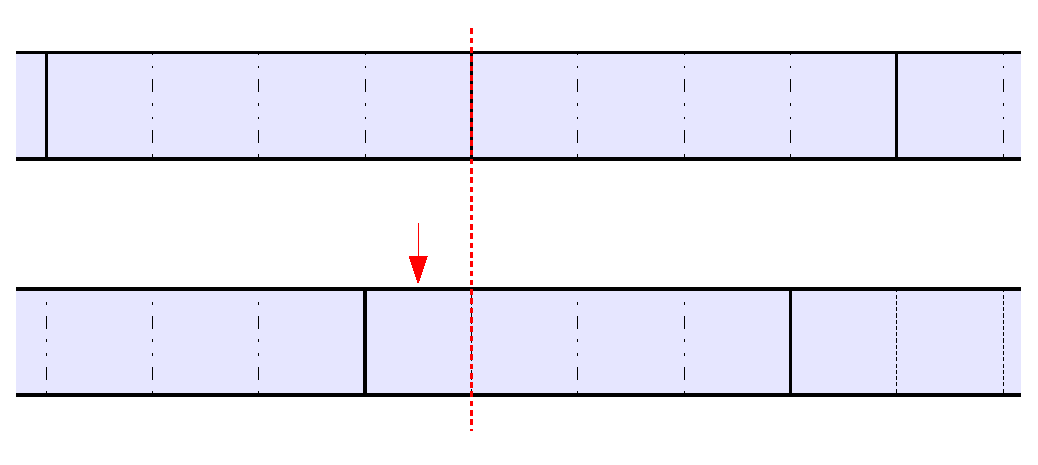
\includegraphics[width=0.5\textwidth]{img/cachelinesplit.eps}
\end{center}
\caption{Example of cache line alignment and cache line split}
\label{fig:cachelinesplit}
\end{figure}

When the programmer can control the allocation of memory himself and the memory should be allocated on the stack, he can easily tell the compiler to align the memory by 16 byte. In gcc this can be done by inserting \texttt{\_\_attribute\_\_ ((aligned(16)))} right after a variable declaration, both for primitives and arrays. The built-in SIMD data types are aligned automatically. Compiler guaranteed alignment of simple data types has the advantage of being totally costless at runtime apart from a possibly increased memory usage. When it is necessary to allocate memory on the heap, the programmer can use special aligning allocators such as \texttt{memalign} or \texttt{valloc} in POSIX compliant operating systems. 

When the programmer has to deal with foreign memory, for example a return buffer from a library call, avoiding misaligned memory accesses will always come with a small processing overhead. When it comes to iterativly processing such a misaligned array, the obvious and probably most practical approach is called \emph{loop peeling} or \emph{loop splitting}. Here, the relevant loop is split up into three parts: the main loop, in which the bulk of the array is processed using SSE instructions, is framed by two loops containing scalar code to process all elements before the first and after the last 16 byte boundary in the array. See Listing~\ref{loop_peeling} for an example. Yet, these additional loops (especially their conditional jumps) amount to increased processing time that can effectivly consume the expected performance gains in some situations. Another simple approach useful for situations with small data that gets created once but is read often would be to copy the data to an aligned memory address.

\begin{code}[caption={Loop peeling example}, label=loop_peeling]
  // Iterate to the first memory address dividable by 16.
  float sum = 0;
  int i = 0;
  for(; (i < count) && (&array[i] % 16 != 0); i++)
    sum += array[i];

  // Vectorized main loop.
  __m128 tmp = _mm_load_ps(&array[2]);
  for(; i < count - (4 - i); i += 4) {
    tmp += _mm_load_ps(&array[i]);
  }
  tmp = _mm_hadd_ps(tmp, tmp);
  tmp = _mm_hadd_ps(tmp, tmp);
  sum += tmp;

  // Add remaining elements.
  for(; i < count; i++)
    sum += array[i];
\end{code}

\subsubsection{Dealing with conditional branches}
\label{conditional_branches} 
The by far hardest hurdle in SSE programming is the transcription of conditional branches. Conditional jumps depending on single values obviously can not exist in data-parallel code and thus need to be replaced by some arithmetic or logical linear statements. For example, consider that we wanted to sum up only those elements of the float vector (refer to Listing~\ref{sse_intrinsics_intro}) that are greater than 5. In a scalar version this would require an \texttt{if} statement within the \texttt{for} loop that, when evaluated to \texttt{true}, would allow the current float to be added to the sum. Getting rid of the conditional jump in scalar C code is possible through evaluating the logical value of a comparison as an integer. Knowing that \texttt{false} is defined to be an integral zero and that \texttt{true} is equal to 1 in most C implementations, we could replace the \texttt{if} statement and therefore the conditional jump with: \texttt{sum += array[i] * (array[i] > 5)}. Comparisons in SSE also define zero as the value of \texttt{false}, but return \texttt{-NaN} as \texttt{true}, which translates to negative ``Not A Number'' or 0xFFFFFFFF, a bitmask that has a 1 at all positions. Thus, whereas scalar C code requires a multiplication to eliminate the conditional jump, SSE takes a bitwise conjunction. See Listing~\ref{sse_blending_intro} for a SSE implementation that calculates the sum of all array elements which are greater than 5.

\begin{code}[caption={Sum of array elements greater than 5}, label=sse_blending_intro]
  __m128 sum = _mm_setzero_ps();
  __m128 five = _mm_set1_ps(5.0f); // (5.0, 5.0, 5.0, 5.0)
  for(int i = 0; i < count; i += 4) {
    __m128 add = _mm_load_ps(&array[i]); // e.g. (1.0, 6.0, 2.0, 8.0)
    __m128 mask = _mm_cmpgt_ps(add, five); // -> (0.0, -NaN, 0.0, -NaN)
    sum += _mm_and_ps(add, mask); // -> (0.0, 6.0, 0.0, 8.0)
  }
\end{code}

If the conditional had an \texttt{else} branch containing a different assignment statement, the SSE code would require two additional bitwise logical operations, namely an \texttt{ANDNOT} for the \texttt{else} assignment and an \texttt{OR} to blend the results of the branches. With SSE4, this triple of bitwise operations has been compacted into a single instruction called \texttt{blendv} (along with other types of blending operations) that merges the bits of two vectors based on a third mask vector. 

In general, performances of vectorized code sections that work around conditionals largely depend on two factors: Probabilities of truth values and the amount of computation done in the related branches. For simple branches such as the assignment statement above it is usually true that a vectorized solution will outperform the scalar version as conditional jumps have a significant impact on performance. Whenever a conditional jump appears in application code, the processor tries to guess what path will be taken and precalculates that branch's results. When the guess turns out to be wrong (\emph{branch misprediction}), the precalculation needs to be discarded and the processor's pipeline needs to be flushed, which can easily stall the processor for a hundred clock cycles. In contrast, vectorized code always evaluates both possible branches and blends the result according to a conditional bitmask, as explained above. As there are no conditional jumps, branch mispredictions become irrelevant. Yet, modern processors feature advanced branch prediction technology and often branch mispredictions get fairly uncommon. In some cases, this may even get to the point where a well predictable condition that determines whether a larger amount of code will be executed or not turns out to be faster than the corresponding vectorized code without condition that will always execute that code. As an extreme example, consider a basic \texttt{if} clause that evaluates to \texttt{true} only once in a thousand runs but then will lead to a considerable portion of code. Here, scalar code may turn out to surpass the performance of its vectorized counterpart. This issue also takes effect in long loops that contain ``early out'' conditionals (e.g. an early \texttt{if}-\texttt{break} group), since the loop needs to be executed until that conditional is \texttt{true} for all vector elements, when it may have canceled the loop for single elements much earlier.

When dealing with long code sections guarded by a conditional, the straightforward approach is to blacklist vector elements that should not take part in the calculation in a blacklist vector. Statements that have no outside effects can then be executed for the whole vector, while those that have outside effects need to be blended depending on the blacklist or need to be performed during or after the unwrapping of the vectors. It may also be possible to omit the blacklist vector and instead directly incorporate the \texttt{NaN} value resulting from the comparison into the calculation. Any operation including a \texttt{NaN} value will always return another \texttt{NaN} value, so the initial \texttt{false} from the comparison will show up at the end of the calculation. However, this may only lead to a small speed-up in comparison to an explicit blacklist vector, mostly due to the blacklist likely having been dropped from cache. Occasionally it may even be feasible to omit the comparison, if the succeeding instructions will always lead to zero or infinity values for those vector elements that originally would have been sorted out by the comparison. However, as this is an arithmetic optimization, it might as well have been done in the original scalar code in the first place.

In case a conditional frequently evaluates to \texttt{false} for all vector elements, the new SSE4 \texttt{ptest} instruction comes to help. This instruction is especially valuable for the above mentioned case of rarely executed code sections after a conditional that is unlikely to be \texttt{true} at all. \texttt{ptest} is the first SSE instruction to operate on the 128 bit value as a whole, it does a bitwise comparison of two \texttt{xmm} registers and returns a scalar \texttt{true} or \texttt{false}. Additionally, Intel provided some helpful convenience intrinsics that test a vector for ``all 1'' or ``all 0'' values which are named \texttt{\_mm\_test\_all\_zeros} and \texttt{\_mm\_test\_all\_ones}. See Listing~\ref{ptest} for two examples of \texttt{ptest} usage.

\begin{code}[caption={Examples of \texttt{ptest} usage},label=ptest]
// Rarely true condition.
__m128 cmp = _mm_cmpgt_ps(a, b);
if(! _mm_test_all_zeros(cmp)) {
  // Rarely executed code.
}

// Test whole vectors for equality.
// Cast intrinsincs do not actually emit an instruction,
// but instead only statically cast the vector types.
int equal = _mm_testc_si128(_mm_castps_si128(a), _mm_castps_si128(b));
\end{code}

\subsubsection{Prefetching \& non-temporal streaming}

When trying to optimize memory throughput of an application, the programmer can manually control cache management with prefetching and streaming. Prefetching, on the one hand, instructs the processor to preload memory into the caches that will be needed soon. This, however, rarely has any effect on performance as modern processors integrate fairly optimized hardware prefetching technology. Yet, in some cases it may yield some improvements when used in the right way. Manual prefetch instructions should always point far ahead in memory (e.g. 500 bytes) and should only be issued when the programmer is absolutely confident that he will need the memory soon and that it has not been cached already. Also he needs to make sure that prefetching does not displace already cached memory segments that are going to be used prior to the prefetched memory, which would result in a performance decline. This is commonly refered to as ``cache thrashing'' and may be considered a rare worst case scenario. Note, that the prefetch instruction is only a hint to the processor which it may or may not obey, in fact, the instruction may not do anything at all, when the processor already is busy loading different segments of memory. Prefetching will always require a fair bit of trial and error and in my experiments resulted in virtually zero performance improvements.

Streaming, on the other hand, is a rather common technique that can significantly increase memory throughput. The \texttt{movnt--} family of SSE instructions (e.g. \texttt{movntps}, meaning ``move non-temporal packed single'') hint the processor that the data that should be moved to memory will not be needed again soon. ``non-temporal'' relates to the temporal characteristic of the before mentioned ``reference of data'' (again, refer to Section~\ref{memory_performance}) which is the foundation of today's cache architecture. When the processor encounters a \texttt{movntps} instruction, it will try to write the data directly to memory and bypass its caches. This has two major advantages over the regular move instructions: First, it is not necessary to read the memory segment to cache first, which results in a noticeable speed-ups if the memory segment has not been loaded to cache already. Second, it will avoid polluting a cache line with pointless data, so that data that may be used again can remain in cache. Though, non-temporal data moves will only avoid caching when used with data big enough to fill up an entire cache line, i.e. at least 64 bytes on most systems. This is due to the fact the processor can only bypass the cache if it is able to use its ``write-combining'' buffers. Apart from that, a common advice seems to be to issue a \texttt{mfence} instruction following the non-temporal streaming instructions, which stalls the processor until any memory operation has completed, in order to ensure that succeeding reads from that memory return the correct data. AMD has provided a helpful summary of how to properly use streaming instructions in their optimization manual~\cite[pp. 106ff, 231ff]{amd2012optimization}. Since SSE has become an industry standard that both Intel and AMD are committed to fully support, most of the information presented in this manual should apply to Intel processors as well.

In order to experience the speed-up of streaming store instructions myself, I wrote three different \texttt{memset} implementations for floating point values. Table~\ref{memset_table} displays results of these experiments using different compiler optimization options (from \texttt{-O0} to \texttt{-O3}). As can be seen easily, the SSE implementation based on simple store instructions turns out to have no impact on performance at all with compiler optimization is turned on, which is likely due to the compiler having auto-vectorized the loop in the scalar version. Streaming store instructions, in constrast, outperform the other implementations by factor 2. It seems impossible for the compiler to determine if the data written to memory is going to be reused soon, thus it does not emit streaming store instructions itself. The code of this benchmark can be found in Appendix~\ref{memset_code}.

\begin{table}[h]
\begin{center}
\caption{Comparison of \texttt{memset} implementations}
\begin{tabular}{lcccc}
\toprule
Implementation & Runtime (s), -O0 & -O1 & -O2 & -O3 \\
\midrule
scalar memset & 0.179 & 0.999 & 0.993 & 0.0987 \\
SSE memset (\texttt{mov} instructions) & 0.100 & 0.102 & 0.103 & 0.100 \\
SSE memset (\texttt{movnt} instructions) & 0.069 & 0.041 & 0.039 & 0.039 \\
\bottomrule
\end{tabular}
\label{memset_table}
\end{center}
\end{table}

\subsection{A word on compiler optimization}
Whenever a programmer chooses to optimize a particular piece of code, he has to be aware of the fact that the compiler --- when used with the right set of command line arguments --- usually may have already created optimal machine code from that code. As a consequence manual code optimization very often will not yield the desired performance improvements but instead may even slow down the application. Besides, manual optimization will always be a time-consuming task and in the end lead to less readable code. Felix von Leitner gave a striking speech~\cite{leitner2009} about compiler optimization at ``Linux Kongress'' conference 2009 in which he emphasizes that it is far more important to learn how compiler optimization works and how to structure code in a way that supports compiler optimization than to try to manually outperform the compiler. He concludes that only when the performance boost ``drastically'' outweighs the decrease in readability, manual optimization really is worth the effort. Again, I would like to point out that the value of manual optimization depends on the very situation. Although on a small scale the compiler will most of the time create fast enough code and manual optimization may not improve performance at all, a human programmer may find optimization measures at a larger scale that speed up execution a lot. The same is true for vectorization: Most modern compilers are able to auto-vectorize specific parts of code such as smaller loops without data dependencies. However, compilers are not able to grasp the complexity of longer loops that could be vectorized as well, for example using branch avoidance techniques as described above.